% =============================================================================
\bloco{1}{General equilibrium, hours and taxes}{Kurlat ch.~9; Romer ch.~2 \,\textbullet\, 25 points}

\questao{(10 points) Objective items.}

\textbf{a)} (3 points) \emph{General equilibrium $\times$ labor supply.} A two-period economy has a fixed capital stock $K$ and no
investment. Households have $u(c)+\psi\ln l$ each period, $u(c)=c^{1-\sigma}/(1-\sigma)$, $\sigma>0$, $\psi>0$, and one unit of time,
$l=1-L$; firms produce $Y=AK^{\alpha}L^{1-\alpha}$ competitively, $0<\alpha<1$. At the equilibrium hours $L\in(0,1)$, the elasticity
$d\ln L/d\ln A$ is:
\begin{alternativas}
\item $1\big/\big[L/(1-L)+\alpha\big]$
\item $(1-\sigma)\big/\big[L/(1-L)+\alpha+(1-\alpha)\sigma\big]$
\item $1\big/\big[L/(1-L)+1\big]$
\item $(1-\sigma)\big/\big[L/(1-L)+1\big]$
\end{alternativas}
\gabarito{B}
\begin{sol}
\passo{equilibrium, period by period}{With $K$ fixed and no investment, $c=Y$; the firm sets $w=(1-\alpha)Y/L$; the household
sets the MRS equal to the wage, $\psi/(1-L)=w\,c^{-\sigma}$. Combining, $\psi L^{\alpha+(1-\alpha)\sigma}/(1-L)=(1-\alpha)(AK^{\alpha})^{1-\sigma}$; the
left side rises from $0$ to $\infty$ on $(0,1)$, so $L$ exists and is unique.}
\passo{log-differentiation}{With $d\ln Y=d\ln A+(1-\alpha)\,d\ln L$, the combined FOC gives $[L/(1-L)]\,d\ln L=(1-\sigma)\,d\ln Y-d\ln L$,
so $d\ln L/d\ln A$ is B. The denominator is positive: the sign is that of $1-\sigma$, and $\sigma=1$ is the knife-edge.}
\passo{distractors}{A holds $c$ fixed (partial equilibrium: no income effect from $c=Y$); D treats output as fixed when hours
move ($d\ln Y=d\ln A$); C makes both mistakes, holding $c$ fixed and treating output as fixed.}
\intuicao{Higher $A$ raises the wage (substitution) and consumption (income, through $c=Y$); with $\sigma>1$ the income effect wins.}
\refbib{Kurlat (2020), \S9.1 (pp.~165--168); Lista 5, Q1.}
\end{sol}

\smallskip
\textbf{b)} (3 points) \emph{General equilibrium $\times$ growth.} In Romer's continuous-time Ramsey model with CRRA coefficient
$\sigma>0$, discount rate $\rho$, population growth $n\ge0$, technology growth $g>0$, depreciation $\delta>0$, $\rho-n-(1-\sigma)g>0$
and $f(\tilde k)=\tilde k^{\alpha}$, $0<\alpha<1$, the steady-state gross saving rate is:
\begin{alternativas}
\item $\alpha(n+g+\delta)/(\rho+\delta+\sigma g)$
\item $\alpha(n+g)/(\rho+\delta+g)$
\item $\alpha(n+g+\delta)/(\rho+\delta+g/\sigma)$
\item $\alpha(n+g+\delta)/(\rho+\delta+g)$
\end{alternativas}
\gabarito{A}
\begin{sol}
\passo{modified golden rule and saving rate}{The Euler equation $\dot{\hat c}/\hat c=[f'(\tilde k)-\delta-\rho-\sigma g]/\sigma$ gives
$f'(\tilde k^*)=\rho+\delta+\sigma g$. Gross investment is $(n+g+\delta)\tilde k^*$ and $\tilde k/f(\tilde k)=\alpha/f'(\tilde k)$, so $s^*=\alpha(n+g+\delta)/(\rho+\delta+\sigma g)$:
A. Also $\alpha-s^*=\alpha[\rho-n-(1-\sigma)g]/(\rho+\delta+\sigma g)>0$: saving is below the Golden-Rule rate because utility is bounded.}
\passo{distractors}{D applies the log-utility Euler equation ($\sigma=1$) to CRRA; C reads $\sigma$ as the intertemporal
elasticity ($r=\rho+g/\sigma$); B makes D's mistake and also counts only net investment $(n+g)\tilde k$. C and D equal A only at $\sigma=1$.}
\intuicao{Growth with curvature ($\sigma g$) raises the required return, so households hold less capital per unit of output.}
\refbib{Romer (2012), \S2.2, \S2.5 and Problem 2.6; Kurlat (2020), \S9.3.}
\end{sol}

\smallskip
\textbf{c)} (2 points, T or F) \emph{General equilibrium $\times$ fiscal policy.} In the Ramsey model on its balanced growth path, a
permanent, unanticipated rise in government purchases per effective worker, financed by lump-sum taxes, lowers consumption
one for one on impact and leaves capital unchanged forever.
\gabarito{T}
\begin{sol}
\passo{proof}{Lump-sum taxes do not enter the Euler equation, so $\tilde k^*$ is unchanged; the resource constraint
$\dot{\tilde k}=f(\tilde k)-\hat c-\hat G-(n+g+\delta)\tilde k$ gives $d\hat c^*/d\hat G=-1$. Capital starts at the old $\tilde k^*$, the new steady-state value; the
constant path $(\tilde k^*,\hat c^*-\Delta\hat G)$ satisfies both equations and the transversality condition, and the saddle path through
a given $\tilde k(0)$ is unique.}
\intuicao{A permanent purchase is a permanent resource loss, absorbed entirely by consumption.}
\refbib{Romer (2012), \S2.7.}
\end{sol}

\smallskip
\textbf{d)} (2 points, T or F) \emph{General equilibrium $\times$ taxes.} In the Ramsey model, a permanent tax at rate $\tau_K\in(0,1)$ on
capital income, whose revenue is rebated lump-sum, leaves the steady-state capital stock unchanged, because the rebate gives
the revenue back.
\gabarito{F}
\begin{sol}
\passo{proof}{Households earn $(1-\tau_K)[f'(\tilde k)-\delta]$, so the Euler equation becomes
$\dot{\hat c}/\hat c=\{(1-\tau_K)[f'(\tilde k)-\delta]-\rho-\sigma g\}/\sigma$ and $f'(\tilde k^*)=\delta+(\rho+\sigma g)/(1-\tau_K)$. Implicit differentiation:
$d\tilde k^*/d\tau_K=(\rho+\sigma g)/[(1-\tau_K)^2f''(\tilde k^*)]<0$, since $f''<0$ and $\rho+\sigma g>n+g\ge0$. The rebate cancels from the
resource constraint: it removes the income effect, not the wedge.}
\intuicao{Saving responds to the marginal after-tax return, which the rebate does not restore.}
\refbib{Romer (2012), Problem 2.10; Kurlat (2020), Exercise 9.6.}
\end{sol}

% -----------------------------------------------------------------------------
\questao{(15 points) Discursive. \emph{General equilibrium $\times$ labor supply $\times$ taxes.} An infinite-horizon economy
without growth: households maximize $\int_0^\infty e^{-\rho t}[\ln c+\psi\ln(1-h)]\,dt$, own the capital and rent it to firms; firms
produce $Y=K^{\alpha}h^{1-\alpha}$; capital depreciates at rate $\delta$; labor income is taxed at rate $\tau$ and the revenue is rebated
lump-sum. Parameters: $0<\alpha<1$, $\rho>0$, $\delta>0$, $\psi>0$, $0\le\tau<1$.}

\textbf{a)} (3 points) Derive the household's optimality conditions (intertemporal and intratemporal), the firm's conditions
and the government budget, and write the equilibrium as a dynamic system in $(K,c)$. Show that hours are a well-defined
function $h(K,c)$ and find its elasticities.
\resolespaco
\begin{sol}
\passo{household}{Budget $\dot k=rk+(1-\tau)wh+T-c$. Shifting consumption across a short interval $\Delta$ at the return $r$:
$u_c(t)=e^{-\rho\Delta}(1+r\Delta)u_c(t+\Delta)$; with $u_c=1/c$ and $\Delta\to0$, $\dot c/c=r-\rho$. Within each instant the MRS equals the
after-tax wage: $\psi c/(1-h)=(1-\tau)w$.}
\passo{firms, government, system}{Firms: $r^K=\alpha K^{\alpha-1}h^{1-\alpha}$, $w=(1-\alpha)K^{\alpha}h^{-\alpha}$; no arbitrage: $r=r^K-\delta$;
government: $T=\tau wh$. With $T$ and $r^KK+wh=Y$ (constant returns) in the budget: $\dot K=K^{\alpha}h^{1-\alpha}-c-\delta K$; Euler:
$\dot c=c(\alpha K^{\alpha-1}h^{1-\alpha}-\rho-\delta)$. Hours solve $\psi c\,h^{\alpha}/(1-h)=(1-\tau)(1-\alpha)K^{\alpha}$, whose left side rises from $0$
to $\infty$ on $(0,1)$: $h(K,c)$ exists, is unique and smooth. Log-differentiating, $[\alpha+h/(1-h)]\,d\ln h=\alpha\,d\ln K-d\ln c$:
\[\frac{\partial\ln h}{\partial\ln K}=\alpha\varepsilon>0,\qquad\frac{\partial\ln h}{\partial\ln c}=-\varepsilon<0,\qquad
\varepsilon\equiv\frac{1}{\alpha+h/(1-h)}=\frac{1-h}{\alpha+(1-\alpha)h}.\]}
\intuicao{$\varepsilon$ blends the Frisch elasticity $(1-h)/h$ with diminishing returns to hours.}
\refbib{Kurlat (2020), \S7.4 and \S9.3; Romer (2012), \S2.2.}
\rubrica{
\item Euler and intratemporal conditions: 1.5 pts (quoted, not derived: max.~0.5 pt).
\item Firms, no arbitrage, government budget: 0.5 pt.
\item System, $h(K,c)$ and its elasticities: 1 pt (unproved signs: 0 for that line).
}
\end{sol}

\textbf{b)} (3 points) Find the steady state. Which ratios and prices does the tax leave unchanged? Find steady-state hours in
closed form and show that they are unique.
\resolespaco
\begin{sol}
\passo{ratios}{$\dot c=0$: $\alpha(K/h)^{\alpha-1}=\rho+\delta$, so $K/h=\bar k\equiv[\alpha/(\rho+\delta)]^{1/(1-\alpha)}$, $K/Y=\alpha/(\rho+\delta)$, $r=\rho$,
$w=(1-\alpha)\bar k^{\alpha}$. $\dot K=0$: $C/Y=1-\delta K/Y=\chi/(\rho+\delta)$, $\chi\equiv\rho+(1-\alpha)\delta$. None depends on $\tau$, $\psi$.}
\passo{hours}{The intratemporal condition with $c=(C/Y)Y$ and $w=(1-\alpha)Y/h$ gives
\[\frac{h^*}{1-h^*}=\Phi\equiv\frac{(1-\tau)(1-\alpha)(\rho+\delta)}{\psi\chi},\qquad h^*=\frac{\Phi}{1+\Phi}\in(0,1),\]
unique as $h/(1-h)$ rises from $0$ to $\infty$ on $(0,1)$; $K^*=\bar k h^*$, $Y^*=\bar k^{\alpha}h^*$, $C^*=(C/Y)\,Y^*$.}
\intuicao{Prescott's formula, with $C/Y$ pinned by impatience and depreciation: the tax sets the level of hours, not the proportions.}
\refbib{Kurlat (2020), \S9.3 and Exercise 7.5; Romer (2012), \S2.5.}
\rubrica{
\item Ratios and prices from the two loci, independent of $\tau$ and $\psi$: 1.5 pts.
\item $h^*$ in closed form, unique: 1.5 pts ($C/Y=1$ assumed: max.~half; hours held fixed: max.~half).
}
\end{sol}

\textbf{c)} (3 points) The tax rises permanently and unexpectedly from $\tau_0$ to $\tau_1\in(\tau_0,1)$. Find the long-run changes in $h$,
$K$, $Y$, $C$, $r$ and $w$ in closed form, and compare the fall in hours with the fall in the net-of-tax rate $1-\tau$.
\resolespaco
\begin{sol}
\passo{hours, scale and prices}{Let $\nu\equiv(1-\tau_1)/(1-\tau_0)\in(0,1)$. By (b), $\Phi$ is proportional to $1-\tau$, so $\Phi_1=\nu\Phi_0$; with
$\Phi_0=h_0/(1-h_0)$, $q\equiv h_1/h_0=\nu/[1-(1-\nu)h_0]$. The denominator lies in $(\nu,1)$, so $\nu<q<1$: hours fall, proportionally less
than $1-\tau$. Locally, $d\ln h^*/d\ln(1-\tau)=1-h^*\in(0,1)$. By (b), $K$, $Y$ and $C$ are fixed multiples of $h$, so each falls by the
same factor $q$; $K/h=\bar k$ is unchanged, so $r=\rho$ and $w$ do not move in the long run.}
\intuicao{The tax shrinks the economy, not its proportions. Hours respond by $1-h^*$, less than the Frisch elasticity $(1-h^*)/h^*$:
consumption falls with them and its marginal utility rises.}
\refbib{Kurlat (2020), \S9.3; Romer (2012), \S2.5.}
\rubrica{
\item $q$ in closed form and $\nu<q<1$, proved: 1.5 pts (ordering without proof: 0 for that line).
\item Same factor for $K$, $Y$, $C$; $r$ and $w$ unchanged, with the reason: 1.5 pts.
}
\end{sol}

\textbf{d)} (3 points) Characterize the transition. Linearize the system in logs at the new steady state, show that it is
a saddle, and find the eigenvalues and the half-life in closed form. Find the impact responses of $c$ and $h$ to first order, compare them with the long-run changes, and draw the paths of $\ln K$, $\ln c$ and
$\ln h$ (deviations from the old steady state).
\resolespaco
\begin{sol}
\passo{log-linear system}{Let $\hat k=\ln(K/K_1)$, $\hat c=\ln(c/c_1)$, $\theta\equiv(1-\alpha)(\rho+\delta)$. Differentiate $\dot K/K=Y/K-c/K-\delta$ and
$\dot c/c=r^K-\rho-\delta$: by (a) and (b), $\partial(Y/K)/\partial(\ln K,\ln c)=[(\rho+\delta)/\alpha](1-\alpha)(\alpha\varepsilon-1,\,-\varepsilon)$,
$\partial(c/K)/\partial(\ln K,\ln c)=(\chi/\alpha)(-1,\,1)$ and $\partial\ln r^K/\partial(\ln K,\ln c)=-(1-\alpha)(1-\alpha\varepsilon,\,\varepsilon)$, so
\[\begin{pmatrix}\dot{\hat k}\\ \dot{\hat c}\end{pmatrix}=J\begin{pmatrix}\hat k\\ \hat c\end{pmatrix},\qquad
J=\begin{pmatrix}\rho+\theta\varepsilon & -(\chi+\theta\varepsilon)/\alpha\\ -\theta(1-\alpha\varepsilon) & -\theta\varepsilon\end{pmatrix}\quad(\varepsilon\text{ at }h_1).\]}
\passo{saddle}{Let $\omega\equiv\alpha+(1-\alpha)h_1\in(\alpha,1)$, so $1+(1-\alpha)\varepsilon=1/\omega$ and $1-\alpha\varepsilon=h_1/\omega>0$. Then $\operatorname{tr}J=\rho$ and
\[\det J=-\frac{\theta\chi}{\alpha\omega}<0,\qquad \mu_{\pm}=\frac{\rho\pm\sqrt{\rho^2+4\theta\chi/(\alpha\omega)}}{2}.\]
Real roots of opposite sign; $K$ is predetermined and $c$ jumps, so the convergent (saddle) path is unique, with speed
$\lambda\equiv-\mu_-$ and half-life $t_{1/2}=\ln2/\lambda$. With $\Lambda\equiv\theta/(\alpha\omega)>(1-\alpha)\delta$, $\lambda$ is the positive root of
$p(x)=x^2+\rho x-\chi\Lambda$, and $p((1-\alpha)\delta)=\chi[(1-\alpha)\delta-\Lambda]<0<\Lambda[\Lambda-(1-\alpha)\delta]=p(\Lambda)$: $(1-\alpha)\delta<\lambda<\Lambda$.}
\passo{impact and paths}{On the stable arm $\hat c=\xi\hat k$, $\xi=(J_{11}+\lambda)/(-J_{12})=\alpha(\rho+\theta\varepsilon+\lambda)/(\chi+\theta\varepsilon)$, with
$\xi-\alpha=\alpha[\lambda-(1-\alpha)\delta]/(\chi+\theta\varepsilon)>0$ and $1-\xi=\alpha(\Lambda-\lambda)/(\chi+\theta\varepsilon)>0$; hours follow
$\hat h=\alpha\varepsilon\hat k-\varepsilon\hat c=-\varepsilon(\xi-\alpha)\hat k$. With $\hat k(t)=-\ln q\,e^{-\lambda t}$ ($K$ starts at $K_0$), relative to the old steady state
\[\ln[x(t)/x_0]=\ln q\,(1-b_xe^{-\lambda t}),\qquad b_K=1,\quad b_c=\xi,\quad b_h=-\varepsilon(\xi-\alpha).\]
On impact $\ln[c(0)/c_0]=(1-\xi)\ln q\in(\ln q,0)$: consumption falls by less than in the long run; $\ln[h(0)/h_0]=[1+\varepsilon(\xi-\alpha)]\ln q<\ln q$:
hours overshoot. The figure uses admissible values.}
\begin{center}
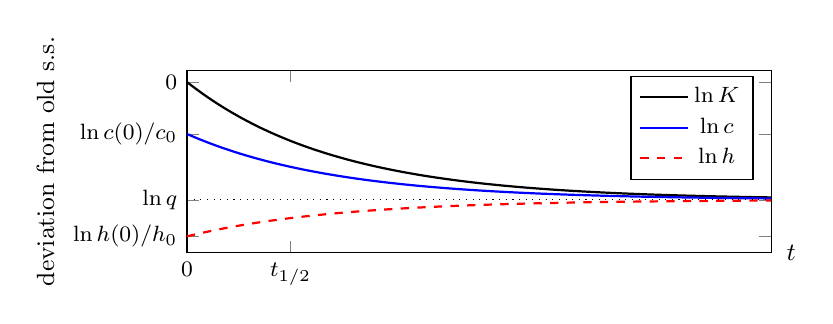
\begin{tikzpicture}
\begin{axis}[width=9cm,height=3.9cm,xmin=0,xmax=25,ymin=-1.45,ymax=0.1,xlabel={$t$},xlabel style={at={(axis description cs:1.01,0)},anchor=west},
  ylabel={deviation from old s.s.},xtick={0,4.4342},xticklabels={$0$,$t_{1/2}$},
  ytick={-1.3108,-1,-0.441,0},yticklabels={$\ln h(0)/h_0$,$\ln q$,$\ln c(0)/c_0$,$0$},
  legend style={font=\footnotesize},legend pos=north east,tick label style={font=\footnotesize},label style={font=\small}]
\addplot[thick,black,domain=0:25,samples=80]{-(1-exp(-0.156319*x))};
\addplot[thick,blue,domain=0:25,samples=80]{-(1-0.559017*exp(-0.156319*x))};
\addplot[thick,red,dashed,domain=0:25,samples=80]{-(1+0.310777*exp(-0.156319*x))};
\addplot[dotted] coordinates {(0,-1) (25,-1)};
\legend{$\ln K$,$\ln c$,$\ln h$}
\end{axis}
\end{tikzpicture}
\end{center}
\intuicao{Capital starts high relative to the new hours, so consumption stays above its new level and the wealth effect
pushes hours below theirs; as capital runs down, consumption falls and hours recover.}
\refbib{Romer (2012), \S2.6 (rate of adjustment and slope of the saddle path); Kurlat (2020), \S9.3.}
\rubrica{
\item Jacobian from the implicit $h$: 1 pt.
\item $\det J<0$, eigenvalues, saddle, half-life: 0.75 pt (saddle without $\det J<0$: 0 for that line).
\item Impact responses signed through $\alpha<\xi<1$, proved: 0.5 pt.
\item Graph (own line): axes; $K$ from $0$, $c$ from $(1-\xi)\ln q$, $h$ below $\ln q$, all tending to $\ln q$: 0.75 pt.
}
\end{sol}

\textbf{e)} (3 points) \emph{Parameter analysis.} Sign the effects of $\tau$, $\psi$ and $\delta$ on $h^*$; on $K^*$, $Y^*$, $C^*$; on $K^*/Y^*$,
$C^*/Y^*$, $r^*$, $w^*$; and on the speed of convergence. Prove each sign, give the limits as $\tau\to1$, $\psi\to\infty$ and $\psi\to0$, and
explain why the speed changes.
\resolespaco
\begin{sol}
\passo{hours and levels}{From (b), $d\ln h^*=(1-h^*)\,d\ln\Phi$: $\partial\ln h^*/\partial\tau=-(1-h^*)/(1-\tau)<0$, $\partial\ln h^*/\partial\ln\psi=-(1-h^*)<0$ and
$\partial\ln h^*/\partial\delta=(1-h^*)[1/(\rho+\delta)-(1-\alpha)/\chi]=(1-h^*)\alpha\rho/[(\rho+\delta)\chi]>0$. For $\tau$ and $\psi$, $K^*$, $Y^*$, $C^*$ move with
$h^*$; the ratios, $r^*=\rho$ and $w^*$ do not move. For $\delta$: $K^*/Y^*=\alpha/(\rho+\delta)$, $C^*/Y^*=1-\alpha\delta/(\rho+\delta)$ and
$w^*=(1-\alpha)\bar k^{\alpha}$ fall; $\partial\ln K^*/\partial\delta=[\alpha(1-\alpha)(1-h^*)\rho-\chi]/[(1-\alpha)(\rho+\delta)\chi]<0$ and
$\partial\ln Y^*/\partial\delta=\alpha[(1-\alpha)(1-h^*)\rho-\chi]/[(1-\alpha)(\rho+\delta)\chi]<0$ because $\chi\ge\rho$; so $C^*=(C^*/Y^*)\,Y^*$ falls too.}
\passo{speed}{By (d), $\lambda=(\sqrt{\rho^2+4D}-\rho)/2$ rises with $D\equiv\theta\chi/(\alpha\omega)$ at given $\rho$; $\tau$ and $\psi$ lower $h^*$, hence $\omega$,
and so raise $\lambda$. For $\delta$:
$\partial\ln D/\partial\delta=1/(\rho+\delta)+(1-\alpha)/\chi-(1-\alpha)h^*(1-h^*)\alpha\rho/[\omega(\rho+\delta)\chi]>0$, as the last term is below
$1/(\rho+\delta)$ ($\alpha\le\omega$, $\rho\le\chi$).}
\par\smallskip\noindent
\begin{minipage}[t]{0.44\linewidth}\vspace{0pt}\centering\setlength{\tabcolsep}{3.5pt}
\begin{tabular}{lccc}
\toprule
Result & $\tau$ & $\psi$ & $\delta$ \\
\midrule
$h^*$ & $-$ & $-$ & $+$ \\
$K^*$, $Y^*$, $C^*$ & $-$ & $-$ & $-$ \\
$K^*/Y^*$, $C^*/Y^*$, $w^*$ & $0$ & $0$ & $-$ \\
$r^*=\rho$ & $0$ & $0$ & $0$ \\
speed $\lambda$ ($t_{1/2}$) & $+\,(-)$ & $+\,(-)$ & $+\,(-)$ \\
\bottomrule
\end{tabular}
\end{minipage}\hfill
\begin{minipage}[t]{0.54\linewidth}\vspace{0pt}\raggedright
\passo{limits}{$\tau\to1$ or $\psi\to\infty$: $h^*\to0$ ($K^*,Y^*,C^*\to0$), $\omega\to\alpha$ and $\lambda\to\bar\lambda\equiv(\sqrt{\rho^2+4\theta\chi/\alpha^2}-\rho)/2$.
$\psi\to0$: $h^*\to1$, $\omega\to1$ and $\lambda\to\underline\lambda\equiv(\sqrt{\rho^2+4\theta\chi/\alpha}-\rho)/2$, the fixed-labor Ramsey speed; so
$\underline\lambda<\lambda<\bar\lambda$. Knife-edge $\delta=0$: $C/Y=1$ and $h^*$ no longer depends on $\rho$.}
\end{minipage}
\intuicao{Prices are pinned by $\rho+\delta$, so $\tau$ and $\psi$ move only the scale. A lower $h^*$ raises the Frisch elasticity
$(1-h)/h$: while consumption is above its new level, hours and output fall more and capital runs down faster; a higher
$\delta$ makes the interest rate react more to a capital gap.}
\refbib{Kurlat (2020), \S7.4 (Frisch elasticity) and \S9.3; Romer (2012), \S2.6.}
\rubrica{
\item Signs proved: 1.5 pts; table: 0.5 pt; limits: 0.5 pt; reading: 0.5 pt (no proofs or no reading: max.~half).
}
\end{sol}
